\chapter{GridWorld: Part 3}
\label{gridworld3}

If you haven't done the exercises in Chapters~\ref{gridworld} and
\ref{gridworld2}, you should do them before reading this chapter.
As a reminder, you can find the
documentation for the GridWorld classes at
\url{http://www.greenteapress.com/thinkapjava/javadoc/gridworld/}.

Part 3 of the GridWorld Student Manual presents the classes that
make up GridWorld and the interactions among them.  It is an
example of object-oriented design and an opportunity to discuss OO
design issues.

But before you read the Student Manual, there are a few more things
you need to know.


\section{{\tt ArrayList}}

GridWorld uses {\tt java.util.ArrayList}, which is an object similar
to an array.  It is a {\bf collection}, which means that it's an
object that contains other objects.  Java provides other collections
with different capabilities, but to use GridWorld we only need {\tt
  ArrayList}s.

To see an example, download
\url{http://thinkapjava.com/code/BlueBug.java} and
\url{http://thinkapjava.com/code/BlueBugRunner.java}.
A {\tt BlueBug} is a bug that moves at random and looks for rocks.
If it finds a rock, it makes it blue.

Here's how it works.  When {\tt act} is invoked, {\tt BlueBug} gets
its location and a reference to the grid:

\begin{code}
    Location loc = getLocation();
    Grid<Actor> grid = getGrid();
\end{code}

The type in angle-brackets (\verb"<>") is a {\bf type parameter}
that specifies the contents of {\tt grid}.  In other words, {\tt grid}
is not just a {\tt Grid}, it's a {\tt Grid} that contains {\tt Actor}s.

The next step is to get the neighbors of the current location.
{\tt Grid} provides a method that does just that:

\begin{code}
    ArrayList<Actor> neighbors = grid.getNeighbors(loc);
\end{code}

The return value from {\tt getNeighbors} is an {\tt ArrayList}
of {\tt Actors}.  The {\tt size} method returns the length of
the {\tt ArrayList}, and {\tt get} selects an element.  So
we can print the neighbors like this.

\begin{code}
        for (int i = 0; i < neighbors.size(); i++) {
            Actor actor = neighbors.get(i);
            System.out.println(actor);
        }
\end{code}

Traversing an {\tt ArrayList} is such a common operation there's a
special syntax for it: the {\bf for-each loop}.  So we could write:

\begin{code}
        for (Actor actor : neighbors) {
            System.out.println(actor);
        }
\end{code}

We know that the neighbors are {\tt Actors}, but we don't know
what kind: they could be {\tt Bug}s, {\tt Rock}s, etc.
To find the Rocks, we use the {\tt instanceof} operator, which
checks whether an object is an instance of a class.

\begin{code}
        for (Actor actor : neighbors) {
            if (actor instanceof Rock) {
                actor.setColor(Color.blue);
            }
        }
\end{code}

To make all this work, we need to import the classes we use:

\begin{code}
import info.gridworld.actor.Actor;
import info.gridworld.actor.Bug;
import info.gridworld.actor.Rock;
import info.gridworld.grid.Grid;
import info.gridworld.grid.Location;

import java.awt.Color;
import java.util.ArrayList;
\end{code}


\section{Interfaces}
\index{interface}

GridWorld also uses Java {\bf interfaces}, so I want to explain what
they are.  ``Interface'' means different things in different contexts,
but in Java it refers to a specific language feature:
an interface is a class definition where the methods have no bodies.

In a normal class definition, each method has a prototype and a
body (see Section~\ref{documentation}).  A prototype is also called a
{\bf specification} because it specifies the name, parameters, and
return type of the method. The body is called the {\bf implementation}
because it implements the specification.

In a Java interface the methods have no bodies, so it specifies
the methods without implementing them.

For example, {\tt java.awt.Shape} is an interface with prototypes for
{\tt contains}, {\tt intersects}, and several other methods.  {\tt
  java.awt.Rectangle} provides implementations for those methods, so
we say that ``Rectangle implements Shape.''  In fact, the first line
of the {\tt Rectangle} class definition is:

\begin{code}
public class Rectangle extends Rectangle2D implements Shape, Serializable
\end{code}

Rectangle inherits methods from {\tt Rectangle2D} and provides
implementations for the methods in {\tt Shape} and {\tt Serializable}.

In GridWorld the Location class implements the {\tt
  java.lang.Comparable} interface by providing {\tt compareTo}, which
is similar to {\tt compareCards} in Section~\ref{compare}.
%
GridWorld also defines a new interface, {\tt Grid}, that specifies
the methods a {\tt Grid} should provide.  And it includes two
implementations, {\tt BoundedGrid} and {\tt UnboundedGrid}.

The Student Manual uses the abbreviation {\bf API}, which stands for
``application programming interface.''  The API is the set of methods
that are available for you, the application programmer, to use.  See
\url{http://en.wikipedia.org/wiki/Application_programming_interface}.


\section{{\tt public} and {\tt private}}

Remember in Chapter~\ref{chap01} I said I would explain why the {\tt
  main} method has the keyword {\tt public}?  Finally, the time has
come.

{\tt public} means that the method can be invoked from other classes.
The alternative is {\tt private}, which means the method can only
be invoked inside the class where it is defined.

Instance variables can also be {\tt public} or {\tt private}, with
the same result: a private instance variable can be accessed only
inside the class where it is defined.

The primary reason to make methods and instance variables private
is to limit interactions between classes in order to manage
complexity.

For example, the Location class keeps its instance variables private.
It has accessor methods {\tt getRow} and {\tt getCol}, but it provides
no methods that modify the instance variables.  In effect, Location
objects are immutable, which means that they can be shared without
worrying about unexpected behavior due to aliasing.

Making methods private helps keep the API simple.  Classes often
include helper methods that are used to implement other methods, but
making those methods part of the public API might be unnecessary
and error-prone.

Private methods and instance variables are language features
that help programmers ensure {\bf data encapsulation}, which means
that objects in one class are isolated from other classes.


\section{Game of Life}

The mathematician John Conway invented
the ``Game of Life,'' which he called a ``zero-player game''
because no players are needed to choose strategies or make decisions.
After you set up the initial conditions, you watch the game
play itself.  But that turns out to be more interesting than it sounds;
you can read about it at
\url{http://en.wikipedia.org/wiki/Conways_Game_of_Life}.

The goal of this exercise is to implement the Game of Life in
GridWorld.  The game board is the grid, and the pieces are Rocks.

The game proceeds in turns, or {\bf time steps}.  At the beginning
of the time step, each Rock is either ``alive'' or ``dead''.  On the
screen, the color of the Rock indicates its status.
%
The status of each Rock depends on the status of its
{\bf neighbors}.  Each Rock has 8 neighbors, except the Rocks along
the edge of the Grid.  Here are the rules:

\begin{itemize}

\item If a dead Rock has exactly three neighbors, it comes to life!
Otherwise it stays dead.

\item If a live Rock has 2 or 3 neighbors, it survives.  Otherwise it dies.

\end{itemize}

Some consequences of these rules:
If all Rocks are dead, no Rocks come to life.  If you start with a
single live Rock, it dies.  But if you have 4 Rocks in a square, they
keep each other alive, so that's a stable configuration.

Most simple starting configurations either die out quickly or reach a
stable configuration.  But there are a few starting conditions that
display remarkable complexity.  One of those is the r-pentomino: it
starts with only 5 Rocks, runs for 1103 timesteps and ends in a stable
configuration with 116 live Rocks (see
\url{http://www.conwaylife.com/wiki/R-pentomino}).

The following sections are suggestions for implementing Game of Life
in GridWorld.  You can download my solution at
\url{http://thinkapjava.com/code/LifeRunner.java} and
\url{http://thinkapjava.com/code/LifeRock.java}.


\section{{\tt LifeRunner}}

Make a copy of {\tt BugRunner.java} named {\tt LifeRunner.java}
and add methods with the following prototypes:

\begin{code}
    /**
     * Makes a Game of Life grid with an r-pentomino.
     */
    public static void makeLifeWorld(int rows, int cols)

    /**
     * Fills the grid with LifeRocks.
     */
    public static void makeRocks(ActorWorld world)
\end{code}

{\tt makeLifeWorld} should create a Grid of Actors and an ActorWorld,
then invoke {\tt makeRocks}, which should put a {\tt LifeRock} at
every location in the Grid.


\section{{\tt LifeRock}}

Make a copy of {\tt BoxBug.java} named {\tt LifeRock.java}.
{\tt LifeRock} should extend {\tt Rock}.  Add an {\tt act} method
that does nothing.  At this point you should be able to run the
code and see a Grid full of Rocks.

To keep track of the status of the Rocks, you can add a new instance
variable, or you can use the Color of the Rock to indicate status.
Either way, write methods with these prototypes:

\begin{code}
    /**
     * Returns true if the Rock is alive.
     */
    public boolean isAlive()

    /**
     * Makes the Rock alive.
     */
    public void setAlive()

    /**
     * Makes the Rock dead.
     */
    public void setDead()
\end{code}

Write a constructor that invokes {\tt setDead} and confirm that
all Rocks are dead.


\section{Simultaneous updates}

In the Game of Life, all Rocks are updated simultaneously; that is,
each rock checks the status of its neighbors before any Rocks
change their status.  Otherwise the behavior of the system would
depend on the order of the updates.

In order to implement simultaneous updates, I suggest that you write
an {\tt act} method that has two phases: during the first phase,
all Rocks count their neighbors and record the results; during the
second phase, all Rocks update their status.

Here's what my {\tt act} method looks like:

\begin{code}
    /**
     * Check what phase we're in and calls the appropriate method.
     * Moves to the next phase.
     */
    public void act() {
        if (phase == 1) {
            numNeighbors = countLiveNeighbors();
            phase = 2;
        } else {
            updateStatus();
            phase = 1;
        }
    }
\end{code}

{\tt phase} and {\tt numNeighbors} are instance variables.
And here are the prototypes for {\tt countLiveNeighbors} and
{\tt updateStatus}:

\begin{code}
    /**
     * Counts the number of live neighbors.
     */
    public int countLiveNeighbors()

    /**
     * Updates the status of the Rock (live or dead) based on
     * the number of neighbors.
     */
    public void updateStatus()
\end{code}

Start with a simple version of {\tt updateStatus} that changes live
rocks to dead and vice versa.  Now run the program and confirm that
the Rocks change color.  Every two steps in the World correspond to
one timestep in the Game of Life.

Now fill in the bodies of {\tt countLiveNeighbors} and
{\tt updateStatus} according to the rules and see if the system behaves
as expected.


\section{Initial conditions}

To change the initial conditions, you can use the GridWorld pop-up
menus to set the status of the Rocks by invoking {\tt setAlive}.
Or you can write methods to automate the process.

In {\tt LifeRunner}, add a method called {\tt makeRow} that creates
an initial configuration with {\tt n} live Rocks in a row in the middle
of the grid.  What happens for different values of {\tt n}?

Add a method called {\tt makePentomino} that creates
an r-pentomino in the middle of the Grid.  The initial configuration
should look like this:

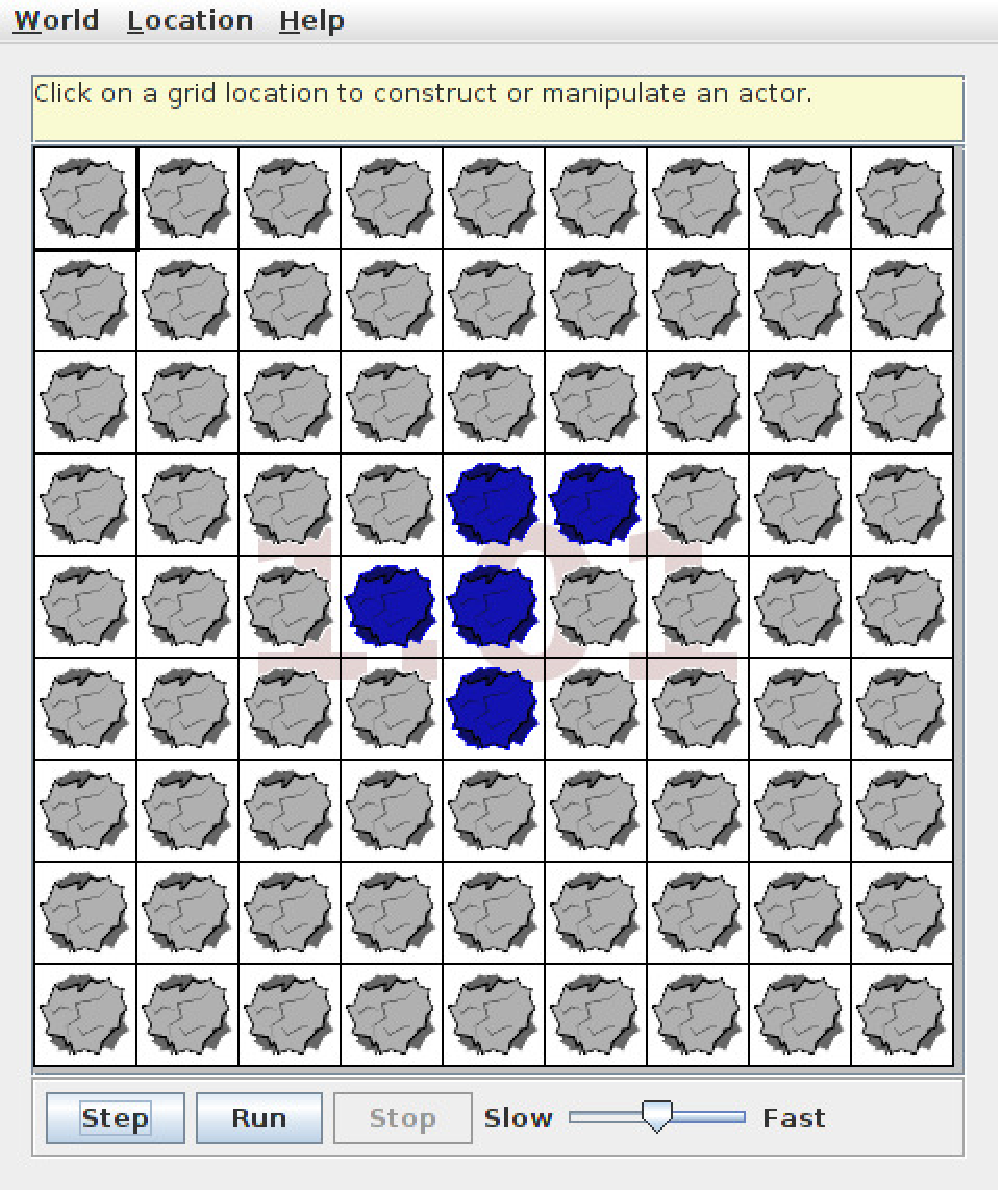
\includegraphics[height=2in]{figs/LifeRunner.pdf}

If you run this configuration for more than a few steps, it reaches the
end of the Grid.  The boundaries of the Grid change the behavior of
the system; in order to see the full evolution of the r-pentomino,
the Grid has to be big enough.  You might have to experiment to find
the right size, and depending on the speed of your computer, it
might take a while.

The Game of Life web page describes other initial conditions that
yield interesting results (\url{http://www.conwaylife.com/}).  Choose
one you like and implement it.

There are also variations of the Game of Life based on different rules.
Try one out and see if you find anything interesting.

\section{Exercises}

\begin{exercise}
Starting with a copy of {\tt BlueBug.java}, write a class definition
for a new kind of {\tt Bug} that finds and eats flowers.  You can
``eat'' a flower by invoking {\tt removeSelfFromGrid} on it.
\end{exercise}

\begin{exercise}
Now you know what you need to know to read Part 3 of the
GridWorld Student Manual and do the exercises.
\end{exercise}

\begin{exercise}
If you implemented the Game of Life, you are well prepared for
Part 4 of the GridWorld Student Manual.  Read it and do the exercises.
\end{exercise}


Congratulations, you're done!
